\documentclass[11pt, twocolumn]{article}

\usepackage{amsmath}
\usepackage{amssymb}
\usepackage{listings}
\usepackage{anyfontsize}
\usepackage{subcaption}
\usepackage{graphicx}
\title{Latent Predicate Networks: Concept Learning with Probabilistic Context-Sensitive Grammars}
\author{Eyal Dechter \& Josh Rule \& Josh Tenenbaum}

\begin{document}
\maketitle

\section{Abstract}
To what extent can the meaning of language be learned from linguistic
data alone?  The sentences that people say contain a great deal of
information about the meaning of linguistic concepts. Most approaches
to semantics assume an explicit knowledge representation formalism
that ties utterances to propositions about things in the world. The
study of linguistic syntax, however, has largely assumed that the
meaning of syntactic structures is encoded directly into the grammar
of a language. For machine learning, extending the grammatical
embedding of meaning to at least some of the linguistic concepts is
attractive because it reduces the problem of automated language
learning to the problem of learning a distribution over naturally
occuring utterances. To what extent is this a feasible approach? Here,
we present a first attempt at the automated induction of probabilistic
context sensitive grammars which we call Latent Predicate Networks
(LPNs), motivated by the idea that the predicates and rules that are
learned correspond to the concepts expressed by utterances. We show
that for a small fragment of sentences expressing relationships
between English number words, we can use hierarchical Bayesian
inference to learn LPNs that can answer simple queries about
previously unseen linguistic concepts within this domain. These
generalizations, we argue, demonstrate LPNs' promise as a tool for
learning and representing conceptual knowledge in language.

% A popular approach in statistical machine learning is to automatically
% find the latent \emph{features} of the data that are most relevant or
% informative. But a latent feature based view of concept learning does
% not match up naturally with the structured symbolic knowledge that
% seems to underlie people's understanding of many domains. How can we
% combine the flexibility, noise tolerance, and computational
% practicality of latent feature based statistical machine learning with
% the symbolic knowledge representations that best capture human
% understanding? Here present a learning model we dub Latent Concept
% Grammars (LCGs) as a proposal. An LCG is a densely connected set of
% probabilistic string rewrite rules over an initially uninterpreted set
% of predicates. When fit to data using a hierarchical Bayesian prior,
% these predicates assume the roles of informative latent concepts. This
% approach allows us to learn knowledge that is stochastic and
% recursively structured while maintaining computational
% tractability. We show how learning in LCGs can be implemented using
% the probabilistic logic programming system PRISM, and we present
% preliminary experiments.

% How do people learn systems of related concepts from
% data?  Consider, for example, a school-age child's knowledge of
% number. This knowledge supports a large number of related operations:
% the child knows which words denote numbers, how to use those words to
% label cardinalities of sets, how to translate between digit
% representations and word representations of number, how to compare
% cardinalities, etc. The child knows how to perform these operations
% over an unbounded set of elements, even though the data that underlies
% this knowledge is small and noisy. Here we propose that such systems
% of related concepts can be learned via hierarchical probabilistic
% inference over probabilistic string rewrite systems (PSRS) -- a mildly
% context-sensitive class of probabilistic string gramamrs that
% corresponds to a restricted fragment of stochastic logic programs
% (SLPs). Specifically, we extend the variational
% expectation-maximization algorithm for Hierarchical Dirichlet PCFGs to
% accomodate PSRSs. This algorithm we present enables a tractible
% compromise between highly restrictive context-free knowledge
% representations and the intractability of performing similar inference
% procedures over general logic programs. Empirically, we show how such
% restricted string rewrite systems can capture non-trivial conceptual
% knowledge and how our algorithm is able to learn such knowledge from
% data.

% \section{Abstract 2}
% What does it mean to understand a concept, and how do people come to
% such an understanding.

\section{Introduction}
The vast majority of the models of concept acquisition that have been
proposed in the artificial intelligence, machine learning and
cognitive science literatures cannot represent the conceptual systems
that even young children learn. Take, for example, the school-age
child's knowledge of number. This child knows that there is no largest
number; that ``one million forty three'' and ``8439''denote numbers
but that ``one million forty billion'' and ``a82bd'' do not; that no
two cardinalities refer to the same quantity but that some number
words refer to the same cardinalities (e.g. ``two thousand'' and
``twenty-one hundred''). Moreover, the child knows how to guage the
approximate number of elements in a collection and how to count this
number exactly. In short, the child's knowledge of number consists of
a complex system of concepts over an unbounded set of entities
(i.e. the numbers). 

Children are not born with this kind of knowledge, and, since number
is a relatively recent cultural invention, nor is it likely that
children possess innate domain specific background knowledge that
makes it easier to acquire. Children only ever see a tiny fraction of
all the numbers they can reason about and this evidence is biased,
noisy, and can be unreliable. 

A fundamental challenge for cognitive science -- and for any field
interested in understanding human-like concept acquisition -- is to
provide a theory of how such complex systems of concepts can be
learned from sparse and noisy data.

People are able to learn about complex systems of related
concepts from small amounts of noisy data. A compelling approach to
understanding such learning is to frame it as Bayesian inference over
probabilistic knowledge bases. Advances in context free grammar
induction in the past couple of decades can be seen as an instance of
this approach, in which

Our goal is to understand how children can obtain semantic knowledge
about a system of concepts from the structure of relavent perceptual
stimuli. How does a child learn that prefixing ``great-'' corresponds
to adding an additional generation in kinship relationships? How does
a child learn that ``just before'' is after ``a while before'' which
is before ``a while after''? How does a child learn that if
Figure~\ref{pairOfApples} is ``a pair of apples'' then
Figure~\ref{singleApple} is a single apple? 

Our proposal is that some interesting fragments of human conceptual
knowledge can be represented as structured relations between
linguistic tokens and other perceptual inputs; that the rules that
define these relations implicitly define the concepts that are
learned; and that these rules can be learned using the tools of
hierarchical Bayesian inference. 

For example, the concept TWENTY SEVEN is defined as the collection of
representations ``27'', ``twenty seven'', ``3 times 9,'' along with a
system of symbolic rules that translate among these representations
and facilitate answered various queries. According to our hypothesis,
the difference between TWENTY EIGHT and TWENTY SEVEN is not that they
are represented in the mind by distinct mental symbols but rather that
the rules that operate on their various representations treat them in
systematically different ways.

This view implies that an attempt to construct a computational account
of concept learning in humans needs to ground out that learning in the
relavent perceptual stimuli. 

Contribution:
\begin{itemize}
\item We present Generate Rewrite Systems (GRS) -- a formalism that borrows
  heavily from Linear Context-Free Rewriting Systems (CITE)
\item We show how GRS, though restricted in representational capactiy,
  can capture substantial cognitively plausible first-order conceptual knowledge 
\item We propose a heirarchical Bayesian model for GRS that provides a coherent framework in which a GRS can be learned given evidence
\item We show how GRS can be transformed into PRISM programs and learned within that probabilstic logic programming system
\item We provide computational experiments that provide evidence that
  our model can provide an account of some kinds of complex conceptual
  knowledge can be inferred from noisy and sparse data
\end{itemize}

\subsection{Related Work}
Our core inference algorithm borrows heavily from recent algorithms for nonparametric PCFG induction, as well as work extending those algorithms to SLPs~\cite{DBLP:conf/emnlp/LiangPJK07,goldwater2006contextual,johnson2006adaptor,cussens2001parameter}. Like Johnson and Liang, we are interested in inferring the most likely grammar given some collection of sentences, and in doing so without a pre-specified limit on the complexity of the grammar. Like Cussens, we are interested in efficiently extending this algorithm to more powerful and expressive formalisms than CFGs.

This work is also closely related to the growing field of semantic parsing. Both are aimed at jointly learning syntactic and semantic information from a body of sentences. Semantic parsers, however, learn separate systems of syntax and semantics, often pairing Combinatory Categorial Grammars of syntax with an explicit logical language of semantics, often the untyped lambda calculus~\cite{berant2013semantic,liang2013learning,kwiatkowski2010inducing}. By contrast, our approach uses a single formalism, the latent predicate network, to describe both which sentences are syntactically valid and what sorts of semantic information those sentence imply. Semantic parsers also typically learn models of semantics by pairing sentences with an explicit logical form or real-world denotation. In our model it is the grammar induction itself which reveals candidate relations between words that are key to capturing their meaning.

More generally, we see this model as helping to strike a balance between expressivity and tractability, bridge the gap between more traditional PCFG grammar induction and program induction over more powerful languages~\cite{dechter2013bootstrap,} (CITATION other P.I. papers).

\section{The Model}

\begin{figure}[t]
		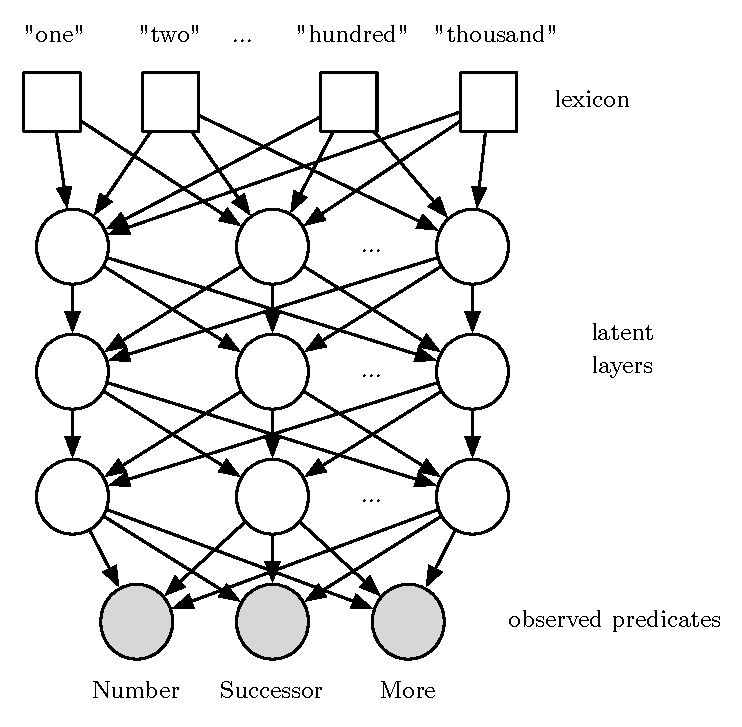
\includegraphics[width=\linewidth]{lpn/lpn.pdf}
		\caption{A schematic LPN where $m = |L|,\, n = |N|-1$,\, arity$(A_i) = 2$, and arity$(S) = 1$.}
		\label{fig:schematic}
\end{figure}

\begin{figure}[t]
		\includegraphics[width=\linewidth]{parseTree/parse.pdf}
		\caption{A possible parse of the sentence ``after twenty five comes twenty six" using a 5-predicate LPN.}
\end{figure}


An LCG is a hierarchical Bayesian model of string tuples. It is an
extension of the Hierarhical Dirichlet PCFG model (HD-PCFG) to
Probabilistic Range Concatenation Grammars (PRCGs). Whereas the
HD-PCFG is a distribution over strings, an LCG is a distribution over
string tuples belonging to one of a set of observable
relations. 

Range Concatenation Grammars (RCGs) are a class of string grammars
that represent all and only those languages that can be parsed in time
polynomial in the length of the target
string~\cite{boullier2005range}. An RCG $G=(N, T, V, P, S)$ is a
5-tuple where $N$ is a finite set of predicate symbols, $T$ is a set
of terminal symbols, $V$ is a set of variable symbols, P is a finite
set of $M \geq 0$ clauses of the form $\psi_0 \rightarrow \psi_1 \dots
\psi_M$, and $S \in N$ is the \emph{axiom}. Each $\psi_m$ is a term of
the form $A(\alpha_1, \dots, \alpha_{\mathcal{A}(A)}$, where $A \in
N$, $\mathcal{A}(A)$ is the arity of $A$, and each $\alpha_i \in (T
\cup V)^*$ is an argument of $\psi_m$. We call the left hand side term
of any clause the \emph{head} of that clause and its predicate symbol
is the \emph{head predicate}.

\textbf{Example:} The following is an RCG for the 3-copy language
$\{www | w \in {a, b}^*\}$:
\begin{alignat*}{3}
&S(XYZ) &&\rightarrow A(X, Y, Z)\\
&A(aX, aY, aZ) &&\rightarrow A(X, Y, Z)\\
&A(bX, bY, bZ) &&\rightarrow A(X, Y, Z)\\
&A(\epsilon, \epsilon, \epsilon) &&\rightarrow 
\end{alignat*}

A string $x$ is in the language defined by an RCG if one can
\emph{derive} $S(x)$. A derivation is a sequence of rewrite steps in
which substrings of the left hand side argument string are bound to
the variables of the head of some clause, thus determining the
arguments in the clause body. If a clause has no body terms, then its
head is derived; otherwise, its head is derived if its body clauses
are derived~\footnote{This description of the language of an RCG
  technically only holds for \emph{non-combinatory} RCGs, in which the
  arguments of body terms can only contain single variables. Since any
  \emph{combinatory} RCG can be converted into a non-combinatory RCG
  and we only consider non-combinatory RCGs here, this description
  suffices.}

We extend RCGs to Probabilistic Range Concatenation Grammars (PRCGs)
by annotating each clause $C_k \in P$ with probabilities $p_k$ such
that for all predicates $A \in N$ $\sum_{k:head(C_k)=A} p_k = 1$. A
PRCGs defines a distribution over strings $x$ by sampling from
derivations of $S(x)$ according to the product of probabilities of
clauses used in that derivation. This is a well defined distribution
as long as no probability mass is placed on derivations of infinite
length; in this paper, we only consider PRCGs with derivations of
finite length, so we need not worry about this requirement.

Now we can describe the model we introduce here, the Latent Concept
Grammar (LCG). We introduce the LCG as a machine learning model to
learn a distribution over instances of relations over strings. Unlike
a PRCG, which places a distribution over terms RCGs consist of a set
of rewrite rules, called clauses, each of which takes a termwhich
operate on a set of terms (predicates applied to arguments) to produce
new terms. Each rewrite rule is of the form:

Suppose we are given some positive instances $y_1, \dots,
y_M$ of relations $R_1, \dots, R_N$. Our model assumes that each
positive instance $y_m=R_n(\vec(x_m))$ is sampled i.i.d from a latent
stochastic grammar (LSG), $\mathcal{K}$. $\mathcal{K}$ consists of
some fixed number $K$ of clauses (i.e. rules) $C_1, \dots, C_K$ over
the $N$ observable relations plus a fixed number of $H$ hidden
relations $T_1, \dots, T_H$. The \emph{architecture} of the model is
the exact specification of the parameters $K$ and $H$ and the clauses
$\mathcal{C}$. To each clause $C_i$ is associated a positive real
weights $\theta_i$.

The clauses of $\mathcal{K}$ are Horn clauses in a first order logic
with string concatenation. We will use PROLOG notation, in which lower
case letters are predicates and constants and uppercase letters are
variables. If two symbols are adjacent it means that the corresponding
strings are concatenated. For example, the following would is a valid
clause: $a(XY, XV) \leftarrow b(X, UV), a(X, X)$. In this rule $a$ and
$b$ are relations with arity two.

Let $C_1, \dots, C_{N(R)} = C(R)$ be the set of clauses whose head is
relation $R$ and let $\Theta_R$ be the set of corresponding
weights. Let $p_R(C_n) \sim \text{Discrete}(\Theta_R)$; that is, $p_R$
is a distribution over the clauses headed by $R$, such that each
clauses is sampled in proportion to its weight parameter.

A positive instance of this relation is sampled from $\mathcal{K}$ by
arbitrarily (i.e. uniformly at random) choosing a relation $R$ and
instantiating that relation by sampling a clause from $p_R$. Recursing
on this procedure for every atom in the body of this clause binds the
variables in the clause's head. 

Given this assumed generative process for the evidence, learning a
program involves inferring the parameter $\theta$ given a prior
probability distribution over their values. We place an independent
Dirichlet distribution over the parameters of every relation. This is
a natural choice that enables us to promote sparse programs, i.e.,
programs in which most of the mass is placed on a small number of
predicates and rules.

\section{Inference}
Inference in hierarchical Dirichlet processes in stochastic grammars
and stochastic logic programs have been well studied. Variational
Expectation-Maximization (VB-EM) is a popular approach, and this is
the algorithm we adopt here. The algorithm is described extensively
elsewhere (CITATION). As we will show in the following section, our
latent stochastic grammar model can be encoded as a stochastic logic
program, so that any VB-EM algorithm for that domain will suffice. 

\section{Implementation}

\lstset{
    language=Prolog,
    basicstyle=\fontsize{9}{10.5}\selectfont\ttfamily
}

\begin{figure}[t]
	\centering
	\begin{minipage}[b]{\linewidth}
A(a, a) :: 0.25. \\
A(b, b) :: 0.3. \\
A(X a, Y a) $\leftarrow$ A(X, Y) :: 0.25. \\
A(X b, Y b) $\leftarrow$ A(X, Y) :: 0.2.
		\subcaption{}
		\label{fig:grammar}
	\end{minipage}
	%\rule[0pt]{0.8\linewidth}{.5pt}
	\begin{minipage}[b]{\linewidth}
		\begin{lstlisting}
values('A', [1, 2, 3, 4],
    [0.25, 0.30, 0.25, 0.20]).

reduce('A'-[[a],[a]],1).
reduce('A'-[[b],[b]],2).
reduce('A'-[A2,B2],3) :- lpn('A'-[X,Y]),
    append(X,[a],A2), append(Y,[a],B2).
reduce('A'-[A2,B2],4) :- lpn('A'-[X,Y]),
    append(X,[b],A2), append(Y,[b],B2).

lpn(P-IN) :- msw(P,V), reduce(P-IN,V).
		\end{lstlisting}
		\subcaption{}
		\label{fig:prism}
	\end{minipage}
	\caption{Possible encodings of the 2-copy language as (\subref{fig:grammar}) an LPN, (\subref{fig:prism}) a PRISM program.}
	\label{fig:copy}
\end{figure}

LPNs can be encoded as a restricted and tractable subclass of Stochastic Logic Programs (SLP). Specifically, we encode LPNs as programs in PRISM PROLOG. PRISM provides probabilistic execution and Bayesian inference over SLPs.

To illustrate the encoding, consider the 2-copy language (CL2) in Figure \ref{fig:copy}. CL2 is a toy language producing two identical strings of $a$s and $b$s, making it mildly context-sensitive. Here, we see four rules concerning a single symbol, $A$, whose total probability sums to unity.

To translate LPNs into PRISM SLPs, we first define the distribution over each symbol. We use the {\tt values} predicate, which takes an atom, in this case the name of the symbol, the values that atom can take on, and the probability of each value. For inference, we initialize the distribution uniformly. For our encoding, each possible value for an atom (or symbol) corresponds to exactly one clause in CL2 where that symbol appears on the left-hand side. There are four clauses for $A$ in CL2, so {\tt values} can take on one of four values, each of whose probabilities corresponds to a rule in CL2.

For each rule in the LPN, we also define a corresponding clause of the {\tt reduce} predicate in our PRISM program. These {\tt reduce} rules are where the actual relations between the left-hand and right-hand side of each rule are encoded. Because PROLOG isn't perfectly declarative, the actual {\tt reduce} clauses are slightly more complex than presented here, reversing the order of the {\tt append} and recursive {\tt lpn} calls based on whether we are sampling or parsing.

To parse or sample a sentence, we call {\tt lpn(P-IN)}, where {\tt P} is the top-level symbol, {\tt IN} is a list of terminal lists, and {\tt -} denotes a pair ({\it e.g.} {\tt lpn('A'-[[a,a,
b,a],[a,a,b,a]])}). A sample or parse begins by probabilistically choosing some rule for the left-hand side via {\tt msw(P,V)} and then recursively reducing the input term using the chosen rule ({\tt reduce(P-IN,V)}). 
\section{Experiments}

\begin{figure}
	\rule{\linewidth}{3in}
	\caption{The Results}
	\label{fig:results}
\end{figure}

\begin{tabular}{l l}
Question & $N_p=4$ \\ \hline
 after twenty comes \underline{\hspace{1cm}}? & twenty one \checkmark \\
 after forty five comes \underline{\hspace{1cm}}? & forty six \checkmark \\
 after forty seven comes \underline{\hspace{1cm}}? & forty eight  \checkmark \\
 after forty nine comes \underline{\hspace{1cm}}? & forty ten $\times$ \\
 after fifty nine comes \underline{\hspace{1cm}}? & fifty ten $\times$ \\
 after sixty one comes \underline{\hspace{1cm}}? & sixty two \checkmark \\
 after sixty three comes \underline{\hspace{1cm}}? & sixty four \checkmark \\
 after sixty four comes \underline{\hspace{1cm}}? & sixty five \checkmark \\
 after sixty five comes \underline{\hspace{1cm}}? & sixty six \checkmark \\
 after sixty nine comes \underline{\hspace{1cm}}? & sixty ten \checkmark \\
 after seventy three comes \underline{\hspace{1cm}}? & seventy four \checkmark \\
 after seventy nine comes \underline{\hspace{1cm}}? & seventy ten $\times$ \\
 after ninety five comes \underline{\hspace{1cm}}? & ninety six \checkmark \\
 before twenty three comes \underline{\hspace{1cm}}? & twenty two \checkmark \\
 before thirty comes \underline{\hspace{1cm}}? & thirty eighty $\times$ \\
 before thirty eight comes \underline{\hspace{1cm}}? & thirty seven \checkmark \\
 before forty one comes \underline{\hspace{1cm}}? & forty \checkmark \\
 before fifty three comes \underline{\hspace{1cm}}? & fifty two \checkmark \\
 before sixty eight comes \underline{\hspace{1cm}}? & sixty seven \checkmark \\
 before seventy two comes \underline{\hspace{1cm}}? & seventy one \checkmark \\
 before seventy three comes \underline{\hspace{1cm}}? & seventy two \checkmark \\
 before eighty five comes \underline{\hspace{1cm}}? & eighty four \checkmark \\
 before ninety two comes \underline{\hspace{1cm}}? & ninety one \checkmark \\
 before ninety three comes \underline{\hspace{1cm}}? & ninety two \checkmark \\
 before ninety five comes \underline{\hspace{1cm}}? &ninety four \checkmark \\

\end{tabular}

\begin{alignat*}{2}
&S(X Y) \leftarrow A_1(X, Y) : 1.0000 \\
&A_1(X Y, U V) \leftarrow A_2(X, U), A_3(V, Y) : 0.5002 \\
&A_2(before, comes) : 0.7316 \\
&A_4(after, comes) : 0.9990 \\
&A_1(X Y, U V) \leftarrow A_3(Y, V), A_4(X, U) : 0.3428 \\
&A_3(one, two) : 0.3993 \\
&A_3(two, three) : 0.2063 \\
&A_3(three, four) : 0.1093 \\
&A_1(X Y, U V) \leftarrow A_1(V, Y), A_4(X, U) : 0.0796 \\
&A_1(X Y, U V) \leftarrow A_1(Y, V), A_2(X, U) : 0.0712 \\
&A_3(four, five) : 0.0734 \\
&A_3(five, six) : 0.0502 \\
&A_3(six, seven) : 0.0355 \\
&A_3(eight, nine) : 0.0290 \\
&A_3(seven, eight) : 0.0271 \\
&A_2(fifty, fifty) : 0.0375 \\
&A_2(thirty, thirty) : 0.0361 \\
&A_2(eighty, eighty) : 0.0339 \\
&A_3(null, one) : 0.0231 \\
&A_2(forty, forty) : 0.0332 \\
&A_2(twenty, twenty) : 0.0310 \\
&A_2(seventy, seventy) : 0.0296 \\
&A_2(sixty, sixty) : 0.0274 \\
&A_2(ninety, ninety) : 0.0260 \\
&A_3(eighteen, nineteen) : 0.0064 \\
&A_3(sixteen, seventeen) : 0.0049 \\
&A_3(eleven, twelve) : 0.0044 \\
&A_3(nine, ten) : 0.0044 \\
&A_3(thirteen, fourteen) : 0.0044 \\
&A_3(fourteen, fifteen) : 0.0039 \\
&A_3(ten, eleven) : 0.0034 \\
&A_2(null, fifty) : 0.0043 \\
&A_3(eighty, null) : 0.0030 \\
&A_3(seventeen, eighteen) : 0.0030 \\
&A_1(X Y, U V) \leftarrow A_2(Y, X), A_3(V, U) : 0.0021 \\
&A_3(nine, sixty) : 0.0025 \\
&A_2(nine, seventy) : 0.0029 \\
&A_3(nine, forty) : 0.0020 \\
&A_1(X Y, U V) \leftarrow A_1(V, Y), A_2(X, U) : 0.0013 \\
&A_2(null, thirty) : 0.0022 \\
&A_2(nine, ninety) : 0.0022 \\
&A_3(twelve, thirteen) : 0.0015 \\
&A_3(fifteen, sixteen) : 0.0015 \\
&A_1(X Y, U V) \leftarrow A_2(V, X), A_3(Y, U) : 0.0008 \\
&A_3(null, comes) : 0.0010 \\
&A_1(X Y, U V) \leftarrow A_1(X, U), A_2(V, Y) : 0.0008 \\
&A_1(X Y, U V) \leftarrow A_1(X, U), A_2(Y, V) : 0.0008 \\
&A_2(twenty, after) : 0.0014 \\
&A_2(sixty, before) : 0.0007 \\
&A_3(nineteen, comes) : 0.0005 \\
&A_4(nine, thirty) : 0.0010 \\
&A_1(X Y, U V) \leftarrow A_1(X, U), A_4(Y, V) : 0.0004 \\
\end{alignat*} \\
\section{Discussion}

%1) Introduction
%  - psychological motivation 
%    - juxtaposing the kinds of knowledge that freebase has and the kinds that children learn
%    - compositional semantic structure --> derive semantics from syntax
%  - what is the contribution?
%     - the use of string rewrite formalisms to capture conceptual knowledge and conceptual learning
%     - to bring tools from computational linguistics to learning semantics
%  - what kind of concept systems are we trying to capture?
%  - why restrict the formalism? 
%     - tractability of inference 
%  - why go beyond context free grammars? 
%     - if they are intractable to learn anyway, why try to go beyond them? 
%  - Related Work
%2) Model
%- stochastic linear context free rewrite systems
%  - model: what is the data? and what is being inferred? what is the prior? 
%  - this can be written as PRISM program, or an SLP. 
%  - inference: variational approximation 
%3) Experiments
%  a) worked example
%  b) Number system (main result)
%  3b) Results
%4) Conclusion
%5) Citations

\end{document}
